% !TeX program = xelatex
% ============================================================
% MEYRUEIS — au fil du temps
% Nouvelle édition corrigée et remise en page
%
% Document principal
%
% Document d'origine
% https://www.calameo.com/read/00500001099e542e47fc5
% ============================================================

\documentclass[a4paper,11pt,twoside]{article}

% ------------------------------------------------------------
% Langue et typographie
% ------------------------------------------------------------

\usepackage[french]{babel}
\usepackage{fontspec}
\setmainfont{Latin Modern Roman}
\usepackage[normalem]{ulem}

\usepackage{fontspec}
\usepackage{graphicx}
\usepackage{lettrine}
\usepackage{microtype}


% Police principale
\setmainfont{TeX Gyre Pagella}

% Police des titres
\newfontfamily\titlefont{TeX Gyre Chorus}

% Présentation générale
\setlength{\parindent}{0pt}
\setlength{\parskip}{0pt}

% Lettrines
\renewcommand{\LettrineFontHook}{}
\setcounter{DefaultLines}{3}
\renewcommand{\DefaultLoversize}{0.15}

% ------------------------------------------------------------
% Mise en page par défaut
% ------------------------------------------------------------
% Format A4 portrait
\usepackage[
    a4paper,
    top=2.00cm,
    bottom=2.00cm,
    left=1.70cm,
    right=1.70cm
]{geometry}

% ------------------------------------------------------------
% Table des matières
% ------------------------------------------------------------

\usepackage{tocloft}
\usepackage[hidelinks]{hyperref}

\renewcommand{\sectionmark}[1]{%
  \markboth{\thesection\enspace–\enspace#1}{}%
}

\renewcommand{\subsectionmark}[1]{%
  \markright{\thesubsection\enspace–\enspace#1}%
}

% Points de conduite sur toutes les lignes
\renewcommand{\cftsecleader}{\cftdotfill{\cftdotsep}}
\renewcommand{\cftsubsecleader}{\cftdotfill{\cftdotsep}}

% Densité des points
\renewcommand{\cftdotsep}{1}

\usepackage{titlesec}

\renewcommand{\cftsecaftersnum}{\enspace–\enspace}
\renewcommand{\cftsubsecaftersnum}{\enspace–\enspace}
\renewcommand{\cftsubsubsecaftersnum}{\enspace\textperiodcentered\enspace}



% --- Espacement et retraits de la TDM ---

% Sections
\setlength{\cftsecindent}{0pt}
\setlength{\cftsecnumwidth}{3.2em}

% Sous-sections
\setlength{\cftsubsecindent}{1.2em}
\setlength{\cftsubsecnumwidth}{3.5em}

% Sous-sous-sections
\setlength{\cftsubsubsecindent}{3.0em}
\setlength{\cftsubsubsecnumwidth}{4.8em}

% Séparateurs après les numéros
\renewcommand{\cftsecaftersnum}{\enspace–\enspace}
\renewcommand{\cftsubsecaftersnum}{\enspace–\enspace}
\renewcommand{\cftsubsubsecaftersnum}{\enspace\textperiodcentered\enspace}

% Espacement vertical
\setlength{\cftbeforesecskip}{0.45em}
\setlength{\cftbeforesubsecskip}{0pt}
\setlength{\cftbeforesubsubsecskip}{0pt}

% ------------------------------------------------------------
% Titres
% ------------------------------------------------------------

\titleformat{\section}
  {\normalfont\Large\bfseries}
  {\thesection\enspace–\enspace}
  {0pt}
  {}

\titleformat{\subsection}
  {\normalfont\large\bfseries}
  {\thesubsection\enspace–\enspace}
  {0pt}
  {}

\titleformat{\subsubsection}
  {\normalfont\normalsize\bfseries}
  {\thesubsubsection\enspace\textperiodcentered\enspace}
  {0pt}
  {}

% ------------------------------------------------------------
% Mise en page des pages
% ------------------------------------------------------------

% Page avec marges
\newcommand{\pagenormale}{%
    \newgeometry{
        top=2.00cm,
        bottom=2.00cm,
        left=1.70cm,
        right=1.70cm
    }%
}

% Page pleine
\newcommand{\pagepleine}{%
    \newgeometry{
        top=0cm,
        bottom=0cm,
        left=0cm,
        right=0cm
    }%
}

% Papier quadrillé type scolaire ancien
\newcommand{\papierquadrille}{%
  \begin{tikzpicture}[remember picture,overlay]
    \draw[
        gray!25,
        line width=0.25pt,
        step=5mm
    ]
      (current page.south west)
      grid
      (current page.north east);
  \end{tikzpicture}%
}

% ------------------------------------------------------------
% Paragraphes en subsubsubsection et subparagraph en subsubsubsubsection
% ------------------------------------------------------------

\usepackage{titlesec}

\setcounter{secnumdepth}{4}
\setcounter{tocdepth}{4}

\titleformat{\paragraph}
  {\normalfont\normalsize\bfseries}
  {\theparagraph}
  {1em}
  {}

\titlespacing*{\paragraph}
  {0pt}
  {3.25ex plus 1ex minus .2ex}
  {1.5ex plus .2ex}

\newcommand{\subsubsubsection}[1]{%
  \paragraph{#1}
}

\setcounter{secnumdepth}{5}
\setcounter{tocdepth}{5}

\titleformat{\subparagraph}
  {\normalfont\normalsize\bfseries}
  {\thesubparagraph}
  {1em}
  {}

\titlespacing*{\subparagraph}
  {0pt}
  {3ex plus 1ex minus .2ex}
  {1.2ex plus .2ex}

\newcommand{\subsubsubsubsection}[1]{%
  \subparagraph{#1}
}

% ------------------------------------------------------------
% Packages
% ------------------------------------------------------------

\usepackage{tikz}
\usepackage{multicol}
\usepackage{titlesec}
\usepackage{array}
\usepackage{tabularx}
\usepackage{wrapfig}
\usepackage{xspace}
\usepackage{etoolbox}
\usepackage{qrcode}
\usepackage{bigfoot}
\DeclareNewFootnote{default}
\setlength{\skip\footinsdefault}{0pt}
\interfootnotelinepenalty=10000

% ------------------------------------------------------------
% Typographie
% ------------------------------------------------------------

%\usepackage{lmodern}
\usepackage{microtype}

\newfontfamily\EBGaramond{EB Garamond 12 Regular}[
    Numbers={OldStyle,Proportional}
]

\newfontfamily\Junicode{Junicode}

% ------------------------------------------------------------
% PDF
% ------------------------------------------------------------

\usepackage{pdfpages}

% ------------------------------------------------------------
% Images
% ------------------------------------------------------------

\usepackage{graphicx}

% ------------------------------------------------------------
% Mise en forme
% ------------------------------------------------------------

\usepackage{enumitem}
\usepackage{xcolor}
\usepackage{tcolorbox}
\usepackage{float}

% Colonnes personnalisées pour les tableaux
\newcolumntype{P}[1]{>{\raggedright\arraybackslash}p{#1}}
\newcolumntype{Y}{>{\raggedright\arraybackslash}X}

\newcommand{\citationblock}[1]{%
    \begin{center}
      \begin{minipage}{0.89\textwidth}
      \itshape #1
      \end{minipage}
    \end {center}
}

\usepackage{afterpage}
\newcommand\myemptypage{%
    \null
    \thispagestyle{empty}
    \addtocounter{page}{-1}
    \newpage
}
% ------------------------------------------------------------
% Réglages généraux
% ------------------------------------------------------------

\setlength{\parindent}{0pt}
\setlength{\parskip}{0.45em}
\setlength{\emergencystretch}{1em}

% ------------------------------------------------------------
% Informations du document
% ------------------------------------------------------------

\newfontfamily\CouvertureFont{Noto Serif}

\newcommand{\Titre}{ALBAN}
\newcommand{\SousTitre}{}
\newcommand{\Edition}{Document ???}
\newcommand{\Infos}{Ce document a été compilé en LaTeX en 2026\\Les images ont été recrées à l'aide de systèmes génératifs\\Pour la version orginale, merci de vous reporter à:\\\DocumentOriginalURL}
\newcommand{\Auteur}{Auteur???}
\newcommand{\Dates}{1622 - 2000}
\newcommand{\edition}{Édition 1.0.0}

\newcommand{\DocumentOriginalURL}{https://matlecurieux.fr/wp-content/uploads/2027/}
\newcommand{\ThisDocumentURL}{https://matlecurieux.fr/wp-content/uploads/2027/}
\newcommand{\ThisDocumentQR}{
    \href{\ThisDocumentURL}{%
          \textbf{Téléchargez ce document au format PDF}
        }
}
\newcommand{\DocumentOriginalQR}{
\href{\DocumentOriginalURL}{%
      \textbf{Consultez le document original}
    }
}
\newcommand{\myemail}{contact@matlecurieux.fr}

% ------------------------------------------------------------
% Pagination
% ------------------------------------------------------------

\pagestyle{plain}

% ------------------------------------------------
% Sections avec date facultative
% ------------------------------------------------

\usepackage{etoolbox}

\newcommand{\sectiondate}[2]{%
    \ifstrempty{#2}{%
        \section{#1}%
        \markboth{#1}{}%
    }{%
        \section[#1 --- #2]{#1}%
        \markboth{#1}{#2}%
    }%
}

%\newcommand{\sectiondate}[2]{%
%    \section[#1\if\relax\detokenize{#2}\relax\else\ --- #2\fi]{#1}%
%    \markboth{#1}{#2}%
%}

\newcommand{\subsectionheader}[1]{%
    \subsection{#1}%
    \markright{#1}%
}


% ------------------------------------------------
% En-têtes et pieds de page
% ------------------------------------------------

\usepackage{fancyhdr}

\pagestyle{fancy}

\fancyhf{}

% Pages impaires
\fancyhead[LO]{%
  \parbox[b]{0.47\textwidth}{\raggedright\small
    \nouppercase{\leftmark}}%
}
\fancyhead[RO]{%
  \parbox[b]{0.47\textwidth}{\raggedleft\small
    \nouppercase{\rightmark}}%
}
\fancyfoot[LO]{Auteur???}
\fancyfoot[RO]{\thepage}

% Pages paires
\fancyhead[LE]{%
  \parbox[b]{0.47\textwidth}{\raggedright\small
    \nouppercase{\rightmark}}%
}
\fancyhead[RE]{%
  \parbox[b]{0.47\textwidth}{\raggedleft\small
    \nouppercase{\leftmark}}%
}
\fancyfoot[LE]{\thepage}
\fancyfoot[RE]{Auteur???}

% Liserés
\renewcommand{\headrule}{%
  {\color{gray!55}\hrule width\headwidth height 0.25pt}%
}
\renewcommand{\footrule}{%
  {\color{gray!55}\hrule width\headwidth height 0.25pt}%
}

\setlength{\headheight}{14pt}

% ------------------------------------------------
% Footnotes
% ------------------------------------------------

\newcommand{\minifootnote}[1]{%
  \footnotemark
  \footnotetext{#1}%
}

% ============================================================
% DOCUMENT
% ============================================================

\begin{document}


% ==============================
% DÉBUT DU LIVRE
% ==============================

\pagenumbering{arabic}
%\setcounter{page}{1}


% ------------------------------------------------------------
% Pages préliminaires
% ------------------------------------------------------------

\pagenumbering{gobble}

\pagenumbering{arabic}


% ------------------------------------------------------------
% Première de couverture : A4 pleine page
% ------------------------------------------------------------
\pagepleine

%\input{pages/001-première-de-couverture}
%\includepdf{pdf/001.pdf}
%\clearpage
%\newpage

% ------------------------------------------------------------
% Retour au format du livre : A4 avec marges
% ------------------------------------------------------------
\pagenormale

%\input{pages/002-page de garde}
%\clearpage

%\input{pages/003-toc}
%\clearpage

% La première page numérotée du document original est la page 1.
\pagenumbering{arabic}
\setcounter{page}{1}


\thispagestyle{plain}

% -----------------------------------------
% TITRE
% -----------------------------------------

\vspace*{12mm}

\begin{center}
%    {\titlefont\fontsize{30}{36}\selectfont
    Alban : montagne druidique !
%}
\end{center}

\vspace{23mm}

% -----------------------------------------
% PREMIER PARAGRAPHE
% -----------------------------------------

{\itshape

Q{uelle}
que soit l'origine du terme « Alban », il est certain
qu'à l'âge de la pierre polie (au néolithique) quelque
2000 ans avant Jésus Christ, des hommes vécurent
sur notre petit plateau et y dressèrent le menhir et le
dolmen qu'on y voit encore. Ceux-ci portent respectivement
le nom de pierre du diable et palet de Notre Dame.
La légende mariale attachée à ces mégalithes est très
pittoresque et fera l'objet d'une relation.

}

\vspace{13mm}

% -----------------------------------------
% DEUXIEME PARAGRAPHE
% -----------------------------------------

{\itshape

D{es}
découvertes faites dans les chantiers d'exploitation
de la région minière qui s'étend d'Ambialet au Roc
de Saint Michel ont établi que des gisements ferreux
étaient exploités dès l'antiquité la plus haute.
Des haches, des lances, des bracelets trouvés nous
révèlent que 12 siècles avant le Christ, les Ligures
parcouraient notre région. Plus tard, les Celtes,
800 ans avant J.C. exploiteront la région albanaise.

}

\clearpage

% ============================================================
% Page 2 — Alban aux temps « gallo-romains »
% Transcription fidèle du document source.
% Mise en page volontairement simple : typographie à définir
% ultérieurement dans le préambule général.
% ============================================================

\thispagestyle{plain}

\vspace*{12mm}

\begin{center}
    {\Large\bfseries Alban aux temps « gallo-romains »}

    \vspace{2mm}
    {\itshape (800 ans avant J.C. -- 400 ans après)}
\end{center}

\vspace{18mm}

\noindent
Des siècles durant, des populations celtiques et romaines se heurtent,
se croisent, cohabitent, finalement s'entendent. Les Gaulois arrivent
jusqu'en Asie mineure (Turquie aujourd'hui) : qu'on se souvienne de la
lettre de Saint Paul aux Galates. Les Romains entraînent leurs légions
jusqu'en Angleterre\ldots{} Chez nous, des débris de poterie, des lampes,
des monnaies attestent la présence de Rome. La Société des Arts et Belles
Lettres du Tarn recevait le 28 juin 1895 de Q. Soulage des lampes romaines
provenant des mines d'Alban. Le 12 mai 1905, on lui présentait une pièce
d'or à l'effigie de Sévère. Le 19 mars 1952, au domaine de Peyre-Augé,
était exhumée\textsuperscript{1} une amphore de forme sphérique du
2ème siècle. Une pièce semblable est au musée de Tours, une autre à
Mende. Le vase gallo-romain « garum » a été plaisamment baptisé
« marmite d'Astérix » : on peut le voir au fond de l'église d'Alban.
Mais à partir de quand Alban « sent-il » vraiment le romain ?

\vfill

\noindent\rule{55mm}{0.4pt}

\vspace{1mm}
{\small\itshape Fouilles de M. Roustan}

\clearpage

% ============================================================
% Page 3 — Alban à l'aube de notre histoire
% Transcription validée du document source.
% Mise en page simple ; typographie et lettrines à traiter
% ultérieurement dans le préambule et le modèle général.
% ============================================================

\thispagestyle{plain}

\vspace*{12mm}

\begin{center}
    {\Large\bfseries Alban à l'aube de notre histoire}

    \vspace{2mm}
    {\itshape (relais gallo-romain)}
\end{center}

\vspace{18mm}

\noindent
Alban fait d'abord partie de la province romaine (Provence).
Avec l'empereur Octave Auguste, il est compris dans l'Aquitaine.
Et après avoir été englobé dans le pays des Ruthènes, le voilà à la
fin du IVème siècle échouant dans la « Civitas Albiensium » limitée
par le Viaur, l'Aveyron, le Thoré, l'Agout.

\par\vspace{9mm}

\noindent
A cette même époque et mêmes limites naît probablement le diocèse
d'Albi. Les découvertes de l'Abbé Hermet de Rodez et de M. Sahue de
Saint Pons tout le long de la route Albi-Béziers, dalles en parties
conservées, ornières encore existantes, vestiges de villas --
statuettes -- disent assez combien les Gallo-romains fréquentaient
cette voie. Alban servit sans doute de « mansio », gîte d'étape ou
relais en même temps qu'il était le débouché naturel de toute la
région minière des environs.

\vfill

\clearpage

% ============================================================
% Page 4 — Alban du IVème siècle à Saint Benoît
% Transcription validée du document source.
% Mise en page simple ; typographie et lettrines à traiter
% ultérieurement dans le préambule et le modèle général.
% ============================================================

\thispagestyle{plain}

\vspace*{12mm}

\begin{center}
    {\Large\bfseries Alban du IVème siècle à Saint Benoît}
\end{center}

\vspace{18mm}

\noindent
Il est normal de penser qu'Alban fut christianisé d'assez bonne heure.
Le christianisme prenait naissance en ville avant de s'étendre à la
campagne. Le mot latin « paganus » a donné en français le doublet
« paysan » et « païen ». L'Albigeois ayant été évangélisé au IVème
siècle par Saint Clair, Saint Amarand, on peut penser que le relais
gallo-romain d'Alban a formé un petit noyau chrétien, peut-être autour
de cet « ALBANUS » qui aurait accolé son nom à celui de Notre Dame.
Les spécialistes de l'histoire religieuse prétendent que les paroisses
sont les plus anciennes -- qui se sont mises sous le vocable de Notre
Dame. C'est le cas d'Alban qui deviendra « Sainte Marie d'Alban ».

\par\vspace{12mm}

\noindent
Les invasions barbares affectent-elles notre petite agglomération ?
La réponse se perd dans les brumes de ces lointaines époques. Un
couvercle de sarcophage dit « Wisigoth » (actuellement appuyé à la
façade ouest de l'église) semble indiquer que le contrecoup de nouveaux
arrivants affecta nos régions. L'intrusion des Arabes dans le midi de
la France y a laissé des traces avec la culture du sarrasin ou blé noir.
Et çà et là quelques individus rappellent par leur teint particulièrement
bronzé et des cheveux très noirs -- le type arabe -- Il est difficile,
à l'heure présente, d'en dire plus.

\vfill

\clearpage

% ============================================================
% Page 5 — Alban aux « siècles bénédictins »
% Transcription validée du document source.
% Mise en page simple ; typographie et lettrines à traiter
% ultérieurement dans le préambule et le modèle général.
% ============================================================

\thispagestyle{plain}

\vspace*{12mm}

\begin{center}
    {\Large\bfseries Alban aux « siècles bénédictins »}
\end{center}

\vspace{18mm}

\noindent
Au VIIème siècle se fonde à Castres le monastère de Saint Benoît.
Un jour, notre petite cité sera, au spirituel, prise en charge par
ces Bénédictins. Alban sera ce qu'on appelle un « prieuré-cure ».
Le titulaire en sera le prieur. Le prieur en titre recevra les revenus
de la paroisse où un jour, il se fera remplacer par un « vicaire
perpétuel » dont il assurera l'entretien par un traitement appelé
« congrue ». En 1545, le monastère disparaîtra et c'est le chapitre
cathédral de Saint Benoît qui nommera le prieur d'Alban et assurera
sa subsistance.

\par\vspace{12mm}

\noindent
Un rarissime parchemin de 1231, un minuscule écrit de deux lignes
garantissant l'authenticité d'une relique -- une pierre sacrée --
sont les plus anciens vestiges de cette époque bénédictine. Des croix
de chemin (le calvaire de Notre Dame d'Outiguet est de 1750), les
croix de consécration de l'église (N.D. d'Alban), les armoiries de
la baronnie d'Alban, rappellent la croix bénédictine (qui s'inscrit
dans un cercle). Il est bien possible que St Michel de Nougaret,
St Michel de la Besse, aujourd'hui disparus aient semblable origine,
mais les documents font défaut.

\vfill

\clearpage

% ============================================================
% Page 6 — Alban aux « siècles bénédictins »
% Transcription réalisée à partir du scan fourni.
% Texte conservé dans sa forme originale ; aucune correction
% grammaticale ou reformulation n'a été effectuée.
% ============================================================

\thispagestyle{plain}

\vspace*{12mm}

\begin{center}
    {\Large\bfseries Alban aux « siècles bénédictins »}
\end{center}

\vspace{18mm}

\noindent
Un bout de parchemin trouvé dans un coin d'un immeuble, aujourd'hui
propriété de M. Délécouls, démontre que, dans la première moitié du
XIII\textsuperscript{ème} siècle, on vénérait ici une relique de
St Vincent, patron des vignerons. Le corps de ce martyr se trouvais
à l'Abbaye de Castres. Selon toute vraisemblance, ce sont les moines
venus de ce monastère qui en apportèrent une relique constituée par
un lambeau de tissu prélevé sur le vêtement de St Vincent. C'est ce
dont fait foi le bout de parchemin en question qu'on peut traduire
« de la tunique du bienheureux Vincent et du tombeau du Seigneur et
du tombeau de N.D. ».

\par\vspace{12mm}

\noindent
Est-ce à dire que ce sont ces bénédictins qui implantèrent ici la
vigne -- comme ce fut le cas pour le Gaillac -- le Champagne ?
Ce n'est pas impossible. Il est vrai que les vignobles sont rares
aux abords d'Alban. Le 12 octobre 1537, noble François Caudières
d'Alban vendait à Bernard Olim de la Mouline à fer une vigne à
Malagousse (parages de l'actuel « Parrot » (archives notariales
d'Albi).

\vfill

\clearpage

% ============================================================
% Page 7 — Alban aux « siècles bénédictins »
% Transcription du document source.
% Texte conservé sans reformulation ni correction.
% ============================================================

\thispagestyle{plain}

\vspace*{12mm}

\begin{center}
    {\Large\bfseries Alban aux « siècles bénédictins »}
\end{center}

\vspace{18mm}

\noindent
Le 19 juillet 1228, entre dans sa « ville d'Albi » son nouvel évêque,
Durant de Beaucaire que Simon de Sully, archevêque de Bourges et
primat d'Aquitaine, appelle « homme de culture, de bonté, d'honneur ».
C'est grâce à lui qu'Alban entre dans l'histoire avec un document écrit
conservé aux archives départementales du Tarn.

\par
En effet, un de ses premiers actes fut de réorganiser le diocèse et
de faire entrer sous son obédience de multiples paroisses réparties
en huit archiprêtrés, dont celui de Négremont. Par accord passé en
1231 avec Adhémar, Abbé de St Benoît de Castres, nous apprenons
qu'une partie de la paroisse de Nougaret, et que la totalité de celle
de Sainte Marie d'Alban, demeurent sous juridiction bénédictine.
C'est donc l'abbaye qui pourvoit au prieuré de Sainte Marie d'Alban.
L'évêque d'Albi n'a d'autre droit que de se faire héberger pour la
visite pastorale ou de percevoir une taxe équivalente appelée
« synodaticum ». « Sancta Maria de Albanio » reste administrativement
compris dans l'archiprêtré de Négremont. Le dernier archiprêtre de
Négremont sera Guillaume de Pressoris. Le pape Eugène IV confirme
le 8 janvier 1438 la décision de l'évêque d'Albi, Robert Dauphin,
supprimant le susdit archiprêtré. Les revenus de la susdite paroisse
serviront à l'entretien de la maîtrise de Sainte Cécile d'Albi.
Alban deviendra chef lieu de claverie, ... mais le douzième siècle
va faire auparavant parler de lui avec l'hérésie cathare. Alerte aux
Albigeois !

\vfill

\clearpage

% ============================================================
% Page 8 — Alban (au XIIème siècle : époque cathare)
% Transcription du document source.
% Guillemets fermants ajoutés à la demande de l'utilisateur.
% Texte conservé sans autre reformulation ni correction.
% ============================================================

\thispagestyle{plain}

\vspace*{12mm}

\begin{center}
    {\Large\bfseries Alban (au XII\textsuperscript{ème} siècle : époque cathare)}
\end{center}

\vspace{18mm}

\noindent
Un moine -- Henri de Lausanne --, un prêtre provençal -- Pierre de
Bruys -- font à Albi le lit à l'hérésie albigeoise. « Le premier
prêche, un christianisme sans le Christ, sans culte, sans sacrements,
sans prêtre, sans église. Le mariage est déclaré « institution
diabolique ». Le second brûle les crucifix, les statues, sous prétexte
d'épuration du culte -- de là naît une décomposition sociale que le
dualisme cathare accentuera. »

\par\vspace{12mm}

\noindent
Le 29 juin 1145, Saint Bernard tonne à la cathédrale d'Albi contre
le dévergondage des mœurs et une piété déliquescente. « Il n'y a
plus que des Chrétiens sans Christ », s'écrie le moine blanc. Ses
invectives n'épargnent pas le clergé. « Les Apôtres étaient la lumière
du monde, vous en êtes les ténèbres. Vous traînez des femmes avec
vous, voire même vous les enfermez avec vous. Comment votre vertu
est-elle en sûreté dans une telle compagnie ? Etre toujours avec
une femme et ne pas pécher est plus difficile que de ressusciter
un mort. »

\par\vspace{12mm}

\noindent
Albi se convertit et le foyer de l'hérésie se déplace pour se fixer
dans la région de Lombers. Qu'advint-il à Alban ? Fut-il contaminé ?
On sait que le vicomte d'Ambialet soutint les Albigeois. Sa vicomté
comprenait Ginestous, La Balme... aux portes d'Alban. Rien ne permet,
à ce jour, d'avancer une certitude à ce sujet.

\vfill

\clearpage


\begin{center}
    {\Large\itshape Alban (au temps des Croisades : XII\textsuperscript{ème} siècle)}
\end{center}

\vspace{1em}

Pour protéger, défendre les « lieux saints » ou les pèlerins s'y
rendant, se fondent des ordres militaires -- Hospitaliers --
Templiers. Ces moines-soldats s'établissent chez nous autant qu'on
puisse le conclure par des documents écrits et des noms de lieux.

\vspace{1em}

Ainsi, le 11 février 1161, Raymond Trencavel donne aux chanoines
de Sainte Cécile l'église et l'hôpital de Carmé (ce qui signifie
les biens des hospitaliers de Montfranc (St Léonard del Carmé).
En 1217, à la suite de difficultés entre le prieur et les frères
de la MAIO de Rayssac avec les hospitaliers du Carmé (Montfranc)
et les chanoines de Ste Cécile, ce fut le prévôt de Vieux et
Bernat de St Sernin qui tranchèrent le différend. En 1447, le
commandeur de Rayssac vend des terres sises à Négremontel
(appartenant aux hospitaliers de Carmésal) à R. Limorin d'Alban.
En 1598, le compoix d'Alban y note la présence d'hospitaliers et
dresse la nomenclature de leurs biens. Un acte du 10 décembre
1682 signale un hospitalier en la personne de Pierre Clergué,
sieur de la Bouyssounade.

\clearpage


\begin{center}
  {\Large\itshape Alban (au temps des Croisades : XII\textsuperscript{ème} siècle)}
\end{center}

\vspace{1em}

Le 5 mai 1688, le visiteur de l'ordre des hospitaliers de St Jean de Jérusalem fait démettre Jean Rollandet, curé de Montfranc de ses droits, sur les biens des hospitaliers du Carmé. En 1767, le commandeur de Rayssac perçoit encore des redevances à Margou. Le 4 septembre 1778, Guillaume Louis Auguste Passemar, de Capriol Saint Maurice, sieur de Cantelosa, Baron d'Alban, vicomte de St André, affirme à Jean Barry le domaine de la « Mare » qui appartient à son épouse, Rose de Clergue.

Les hospitaliers s'implantent donc dans la région d'assez bonne heure et au cours des siècles, ils auront beaucoup de biens fonciers dans le coin : notez Alban, Montfranc, Rayssac, Carmenel, la Maie, la Font de Carmé, le mas de Carmé, la Boyssounade. Et si « Carmenel » signifie « le petit Carmé », on voit combien ont prospéré des hospitaliers établis d'abord à Montfranc (St Léonard du Carmé) et essaimant dans la région.

Notons que le mot « maio » qui semble bien signifier maison ou communauté de frères hospitaliers, s'explique très bien au voisinage de la font (de Carmé) et du mas de Carmé, ce dernier disparu.

Par la suite, une dame ou demoiselle a fait graver son écu avec une maille (ou fils entrecroisés) sur une pierre avec en accolade -- qui sert de margelle à la font de la maye -- Est-ce cette Rose de Clergue qui devint l'épouse du Passemar, sieur de Cantelauze, baron d'Alban -- ci-dessus nommé ?



\clearpage



\begin{center}
  {\Large\itshape Alban (au temps des Croisades : XII\textsuperscript{ème} siècle)}
\end{center}

\vspace{1em}

Le 5 mai 1688, le visiteur de l'ordre des hospitaliers de St Jean de Jérusalem fait démettre Jean Rollandet, curé de Montfranc de ses droits, sur les biens des hospitaliers du Carmé. En 1767, le commandeur de Rayssac perçoit encore des redevances à Margou. Le 4 septembre 1778, Guillaume Louis Auguste Passemar, de Capriol Saint Maurice, sieur de Cantelosa, Baron d'Alban, vicomte de St André, affirme à Jean Barry le domaine de la « Mare » qui appartient à son épouse, Rose de Clergue.

Les hospitaliers s'implantent donc dans la région d'assez bonne heure et au cours des siècles, ils auront beaucoup de biens fonciers dans le coin : notez Alban, Montfranc, Rayssac, Carmenel, la Maie, la Font de Carmé, le mas de Carmé, la Boyssounade. Et si « Carmenel » signifie « le petit Carmé », on voit combien ont prospéré des hospitaliers établis d'abord à Montfranc (St Léonard du Carmé) et essaimant dans la région.

Notons que le mot « maio » qui semble bien signifier maison ou communauté de frères hospitaliers, s'explique très bien au voisinage de la font (de Carmé) et du mas de Carmé, ce dernier disparu.

Par la suite, une dame ou demoiselle a fait graver son écu avec une maille (ou fils entrecroisés) sur une pierre avec en accolade -- qui sert de margelle à la font de la maye -- Est-ce cette Rose de Clergue qui devint l'épouse du Passemar, sieur de Cantelauze, baron d'Alban -- ci-dessus nommé ?



\clearpage

\documentclass[12pt,a4paper]{article}

\usepackage{fontspec}
\usepackage[french]{babel}
\usepackage{geometry}
\usepackage{microtype}

\geometry{
  top=2.5cm,
  bottom=2.5cm,
  left=2.5cm,
  right=2.5cm
}

\setlength{\parindent}{1.2em}
\setlength{\parskip}{0.65em}

\begin{document}

\setcounter{page}{11}

\begin{center}
  {\Large\itshape Alban (au temps des Croisades)}
\end{center}

\vspace{1em}

L'époque des croisades a laissé -- grâce aux hospitaliers -- quelques souvenirs à Alban et dans son voisinage. Jusqu'à ces derniers temps -- dans l'enclos de St Léonard du Carmé (Montfranc) -- la tombe de l'Abbé Paul Routoulp, curé de Notre Dame d'Alban de 1763 à 1791, était surmontée d'une croix de pierre en forme de croix de Malte, insigne des Hospitaliers de St Jean de Jérusalem.

Mais un monument qui lui, est resté, c'est l'église de Notre Dame de la Garde. Une tradition orale dit qu'un pèlerin de Terre Sainte ait fait vœu de bâtir une chapelle à Notre Dame de la Garde, s'il revenait sain et sauf de son voyage après avoir essuyé maintes tempêtes. Revenu chez lui, il réalisait sa promesse. Et déjà en 1290, le pape Nicolas II accordait des indulgences à qui se rendait à ce sanctuaire. Les archives conservent le souvenir des pieuses démarches des Consuls d'Albi à la dévote chapelle à l'occasion de la peste de 1518. Au début du XIX\textsuperscript{ème} siècle, une grande dame, Louise de Bayne de Rayssac faisait à son amie Eugénie de Guérin, le récit de son pèlerinage matinal à Notre Dame de la Garde à la Pentecôte de 1837. Peut-être y eut-il de plus illustres pèlerins, mais nous l'ignorons.

\end{document}

\clearpage

% Page 12 — Alban « la féodale »
% Fragment à intégrer au document principal avec \input{012.tex}

\begin{center}
  {\Large\itshape Alban « la féodale »}
\end{center}

\vspace{1.5em}

\noindent
\lettrine{I}{l} est difficile d'établir les contours précis de l'Alban primitif.
En se référant à ce qui existait encore en 1598, nous pouvons faire une
reconstitution approximative d'une petite cité féodale entourée de murs
crénelés donnant sur des fossés extérieurs qui la protégeaient contre un
ennemi éventuel. Le centre en pouvait être l'actuelle place de l'église.
On accédait à notre bourg par la porte si l'on venait d'Albi, et par
« lou pourtal haut » si l'on arrivait de Montfranc. C'est non de la
« carreprolo » que se dressait dans une maison à trois étages la chambre
du guetteur. Il y avait encore en 1598 deux maisons à deux étages.
Les autres demeures devaient être modestes. Des groupes de jardins
« ourtalissos » jouxtaient les deux portails d'accès. On y pouvait voir
un « fourmial », un « grand carrairé », un « fieyrol ». La « fountanario »
mise à part, il est difficile de localiser la « fountetto si passado »,
loui mouli dal Bin, la « coumbo de bedel ». Les gens aujourd'hui ont
perdu le souvenir de bien des lieux aux noms charmants. A noter pour
les curieux et les poètes que fountaourio signifie « source d'or ».
Pourquoi ? La « carragrolo » est le chemin d'Alban à Peyreblanque,
près du pâtissier Rémy.

\clearpage

\begin{center}
  {\Large\itshape Alban « la féodale » -- XIII\textsuperscript{ème} siècle}
\end{center}

\vspace{1.5em}

\noindent
\lettrine{A}{u} civil -- comme Nougaret -- Alban est englobé dans le Comté
de Castres. Il se pourrait qu'à la suite de la croisade des Albigeois,
Philippe de Montfort, neveu du trop fameux Simon, ait donné en 1229,
à la mort de son oncle, la Seigneurie d'Alban à l'Abbaye Saint Benoît
de Castres. C'est ce début du XIII\textsuperscript{ème} siècle que les
vicomtes d'Albi et d'Ambialet accordent des franchises aux villes de
leur ressort. Alban a dû posséder, dès cette époque, une ébauche
d'organisation municipale en la personne de deux consuls. Au
XVII\textsuperscript{ème} siècle, ces magistrats sont choisis par le juge
mage de la sénéchaussée de Castres sur une liste de quatre candidats
présentés par les électeurs d'Alban.

\vspace{0.8em}

\noindent
\lettrine{L}{a} justice est rendue par l'Abbé de Castres. Mais, au
XIV\textsuperscript{ème} siècle, il y a concurremment le sénéchal qui
l'exerce. Assez souvent, les ressortissants préféreront la justice
d'Eglise.

\vspace{0.8em}

\noindent
Deux bulles de Clément IV en 1266 et 1267 confirmant l'accord de 1231
entre l'évêque d'Albi et l'Abbé de Castres stipulent que St Michel de
Nougaret comme Ste Marie d'Alban demeurent sous juridiction
bénédictine. En 1274, Pierre Raymond de Janes y exerce la fonction
de notaire. En juin 1286, un grand seigneur ecclésiastique,
l'archevêque de Bourges métropolitain d'Albi passe par Alban, venant
de Montfranc où il a dit la messe chez les Hospitaliers à St Léonard
du Carmé. C'est avec une forte escorte qu'il traverse Alban pour se
rendre à Ambialet.

\clearpage

\begin{center}
  {\Large\itshape Alban à l'heure des troubadours -- XIII\textsuperscript{ème} siècle}
\end{center}

\vspace{1.5em}

\noindent
\lettrine{S}{ur} le portail nord de N.D. de Paris, est sculptée dans la
pierre l'histoire de Théophile qui vendit son âme au diable et fut
sauvé par la Vierge. Entre les deux guerres mondiales, un professeur
de Sorbonne et ses étudiants, penchés sur le récit qu'en avait fait
au XII\textsuperscript{ème} siècle le poète Rutebeuf, y trouvèrent le
chemin de la foi. Gustave Cohen passa au catholicisme, un de ses
élèves se fit dominicain, une autre entra au cloître ? Alban n'a pas
eu la même chance. C'est de bouche à oreille qu'est venue jusqu'à
nous une semblable légende, mais combien plus pittoresque que celle
de Paris. Quel troubadour l'inventa, la chanta ? Est-ce un descendant
de ces « Brossard d'Alban », d'origine normande ? L'un d'eux fut le
grand argentier de Philippe le Bel. Veut-il s'implanter dans le midi
comme le fit l'un d'entre eux en 1950 ? Est-ce un ancêtre de ce
« Pierre d'Alban », cabaliste cité par Pierre Benoît dans
« La Châtelaine du Liban » ? Peu importe le nom de ce marchand de
rêve, qui allait jouant de sa viole, chantant les amours de quelque
Tristan et Iseult, ou mieux, célébrant avec ferveur cette Madone de
chez nous, plus suave que le parfum de violette, plus délectable que
le miel le plus savoureux et finalement se laissa prendre à la
« caresse de ces mots ». « Notre Dame »... que de foyers durent
l'entendre.

\clearpage

% Page 16 — Illustration de Pierre d'Alban
% Fichier image associé : Pierre_d_Alban.png

\begin{center}
  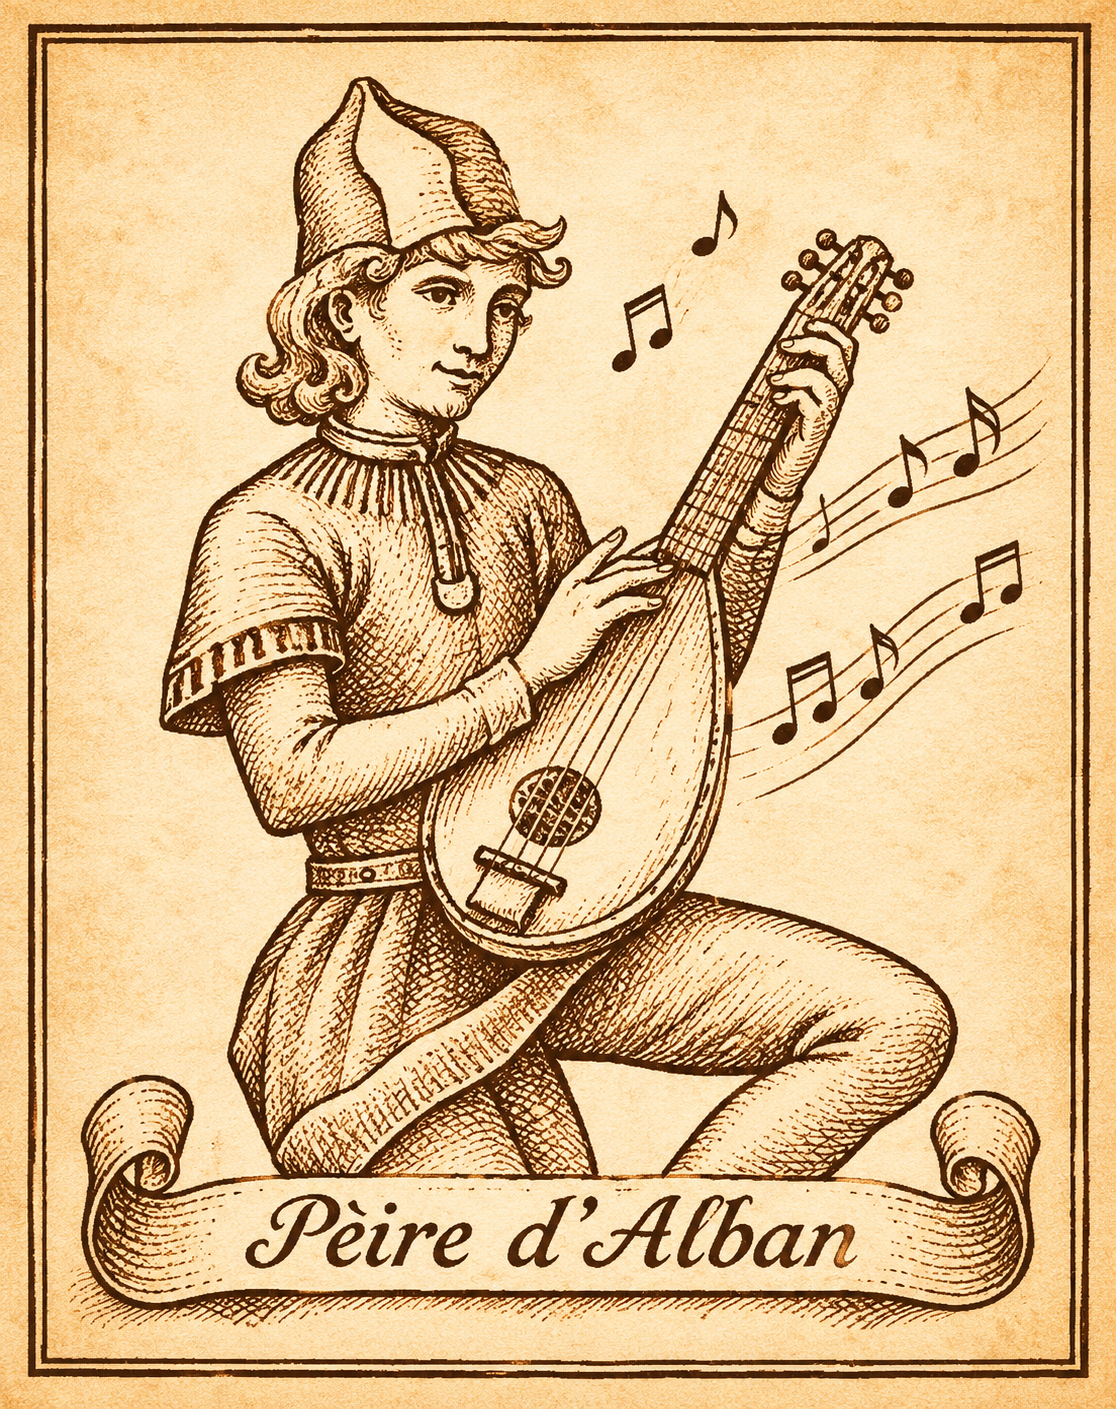
\includegraphics[
    width=0.78\textwidth,
    height=0.85\textheight,
    keepaspectratio
  ]{imgs/004}
\end{center}

\clearpage

\newpage

\begin{center}
    {\Large\itshape Alban à l'heure du troubadour « Pierre d'Alban »}
\end{center}

\vspace{1.2em}

\lettrine[lines=3,lhang=0.1,nindent=0em]{N}{otre} poète ambulant n'eut que l'embarras du choix pour faire retentir sa chanson dans les « castels » du voisinage. Sa devise « audenti succedit opus » -- l'audace paie -- dut l'amener au château de Paulin, à celui de Miolles où les chevaliers de Matha devaient s'illustrer par un des leurs, Saint Jean de Matha. La Tapie dut avoir sa visite. Un sieur de Pujol au XIV\textsuperscript{e} siècle y sera qualifié de « plus fort pétardier de France ». Il est probable qu'il fut accueilli à Massals où les Brandouin ont laissé gravés dans la pierre les panaches de leurs armes. Les châteaux de Nougaret, d'Alban, de Saint-André, de Coupiac durent l'accueillir. S'il s'aventura sur les berges du Tarn, il fut peut-être l'hôte des « de Sales » dont un cousin devient évêque de Genève, le célèbre Saint François de Sales. Poussa-t-il jusqu'à la demeure du vicomte d'Ambialet et chez les moines bénédictins du prieuré voisin ? C'est vraisemblable. Quel que soit le seigneur de haut lignage, quelle que fut la dame « de haute cuisse » qui ait allumé cette étoile filante au ciel de l'Albigeois, nous avons la chance qu'un écho de la voix de charme de notre troubadour ait récemment retenti grâce à Annick Roche dont voici le récit\ldots

\clearpage

\newpage

\begin{center}
    {\Large\itshape Alban en sa « légende dorée »}
\end{center}

\vspace{1.2em}

\lettrine[lines=3,lhang=0.1,nindent=0em]{I}{l} y a de cela fort longtemps, vivait en son castel Alain de Nougaret, seigneur très redouté, baron d'Alban. Aujourd'hui, le château a complètement disparu. Il est mentionné en des actes notariés de 1248. On peut retrouver quelques traces du hameau de Nougaret au « Roc des Anglais » où la roche se voit taillée à angles droits. Un document du XV\textsuperscript{e} siècle situe le château de Saint Michel de Nougaret entre le ravin de Nougaret et le chemin d'Alban à Saint André. La ferme dite du « Castellàs » pourrait bien être un témoin de l'édifice aujourd'hui introuvable\ldots La réputation d'Alain de Nougaret était rien moins que bonne. On lui prêtait des pillages d'églises, des assassinats de pèlerins venus faire leurs dévotions au sanctuaire de Notre Dame d'Alban et d'ailleurs\ldots Notre Dame de Bon Secours de Villefranche, Notre Dame de la Garde par delà Saint Jean de Janes. Ce seigneur quelque peu bagarreur ne se contentait pas de détrousser les pieuses personnes que la dévotion attirait en ces lieux. Les paysans qui travaillaient ses propres terres n'étaient pas à l'abri de ses mauvais traitements. Comment de telles dépravations pouvaient-elles se concilier avec des pratiques de dévotion à l'égard de la Madone ? Bien malin qui le dira\ldots

\clearpage

\newpage

\begin{center}
    {\Large\itshape Alban en sa « légende dorée »}
\end{center}

\vspace{1.2em}

\lettrine[lines=3,lhang=0.1,nindent=0em]{M}{ais} c'est un fait, le Seigneur de Nougaret, baron d'Alban, n'aurait pas passé une journée sans invoquer Notre Dame d'Alban -- « débonnaire Dame, plus savoureuse que le miel, plus suave que le parfum des violettes ». Ainsi s'exprimait le langage du temps\ldots Et ce dévot serviteur de Notre Dame n'en continuait pas moins ses vilenies. Hélas, les méfaits d'Alain devinrent si nombreux que bientôt, la révolte gronda dans la baronnie. Les paysans soulevés contre lui l'enfermèrent dans la prison de son propre château. Tête basse et l'œil triste, notre baron s'attendait à être pendu d'un moment à l'autre par ses propres sujets irrités. Mais Satan survint. Il promit la liberté. Une seule condition était exigée : livrer son âme au démon pour l'éternité. Le contrat tout prêt était à portée de la main. On n'avait qu'à signer et l'affaire était réglée. Troublante alternative que celle d'une mort imminente ou celle d'une liberté si chèrement achetée. Les Anglais prétendent que si l'on soupe avec le diable, il faut prendre une longue cuiller. Autant dire que discuter avec Satan, c'est être perdu.

\clearpage

% Page 19 — Alban en sa « légende dorée »
% À intégrer dans le document principal (XeLaTeX).
% Nécessite le package lettrine.

\begin{center}
    {\Large\itshape Alban en sa « légende dorée »}
\end{center}

\medskip

\lettrine[lines=2]{M}{ais} devinez donc ce qui vient d’arriver ? Alain de Nougaret,
Baron d’Alban a signé le contrat qui le livre à Satan pour l’éternité.
Lucifer regarde avec un sourire féroce celui qui vient de se laisser prendre
à ses infernales propositions. Oui, c’est vrai, Alain a signé de son sang
le parchemin diabolique, mais Alain est libre. Si vous pensez peut-être
qu’il va profiter de cette liberté pour faire le bien et se racheter ?
Trois fois hélas ! c’est de nouveau une vie de pillage qui recommence.
Et de jour et de nuit, il est à l’affût de quelque victime. Satan a bien
fait les choses. Alain de Nougaret arpente les chemins du crime, dévore
les routes spacieuses qui mènent à l’enfer éternel. Mon Dieu, mon Dieu,
jusqu’où ira-t-il ? Et la Madone de pitié l’aurait-elle définitivement
abandonné ?

\medskip

\lettrine[lines=2]{N}{on}, la Vierge n’abandonne jamais, comme vous allez le voir,
mais la folie des hommes peut aller loin. Et c’est par une soirée de ripaille
et de débauche qu’Alain va être pris dans les filets d’une miséricorde infinie.
Il festoie en son château de Nougaret tandis que ses paysans à nouveau révoltés
assiègent son repaire et de toutes parts y mettent le feu. Femmes, enfants,
domestiques, tout le monde va périr dans les flammes et lui-même sera grillé.
Qui l’eût cru ? Alain est le seul à s’être échappé du château qui flambe et
le voilà meurtri mais bien vivant au milieu d’un fourré… Alors…

\clearpage

% Page 20 — Alban en sa « légende dorée »
% À intégrer dans le document principal (XeLaTeX).
% Nécessite le package lettrine.

\begin{center}
    {\Large\itshape Alban en sa « légende dorée »}
\end{center}

\medskip

\lettrine[lines=2]{A}{lors}, comme le prodigue de la parabole, le malheur touche son âme,
les larmes jaillissent de ses yeux, et du cœur à ses lèvres monte la prière
à la Madone, cette oraison qu’on apprend tout petit sur les genoux d’une
pieuse mère :

\begin{center}
    O Notre Dame d’Alban -- Mère très aimée\\
    Tenez-nous toujours blottis contre votre cœur immaculé\\
    Afin que nous croissions, de jour en jour, en sagesse\\
    Et dans la crainte du Seigneur.
\end{center}

\medskip

\lettrine[lines=2]{A}{lain} n’est plus Alain. Alain est converti et le voici au soir d’une
terrible journée, à la nuit noire, demandant asile et protection au prieuré
bénédictin de Notre Dame d’Alban. Comment les disciples de Saint Benoît
auraient-ils pu se récuser devant les larmes et les prières d’un pareil
larron repentant ? Comment refuser pareil novice ? On tenta l’aventure
charitablement. Frère Alain prit donc le froc monacal. En attendant une
conversion totale et bien affermie, il rendrait à ses frères quelques menus
services, balayant la chapelle, désherbant le cimetière, arrosant le potager.
On verrait par la suite. Et la suite dépassa les espoirs les plus optimistes.
Qui eût pu, sous cette bure pacifique, reconnaître le terrible sire de
Nougaret ? Certainement pas les enfants…

\clearpage

% Page 22 — Alban en sa « légende dorée »
% À intégrer dans le document principal (XeLaTeX).
% Nécessite le package lettrine.

\begin{center}
    {\Large\itshape Alban en sa « légende dorée »}
\end{center}

\medskip

\lettrine[lines=2]{L}{es} enfants venus faire leurs dévotions à la chapelle de Saint Joseph,
racontaient aux bons moines qui les recevaient, et ce, avec joie et un brin
de malice, les bruyants ébats qu’ils prenaient jusque dans les ruines du
vieux « castel ». Ils n’y rencontraient plus « le très méchant Alain de
Nougaret » dont on parlait encore aux veillées d’hiver comme d’un terrible
croquemitaine. « Il faut prier pour les pécheurs », se contentait de répondre
avec humilité le religieux pénitent.

\medskip

\lettrine[lines=2]{L}{es} paysans eux-mêmes qui venaient recommander leurs bestiaux à la
protection de Saint Roch dont la chapelle faisait pendant à celle de
Saint Joseph, ne se doutaient pas de la personnalité de frère Alain.
Il leur arrivait même de parler avec une vindicative rudesse de leur ancien
maître. « Heureusement qu’on a grillé Alain de Nougaret comme un poulet
et vraisemblablement il doit encore griller en enfer, car il avait vendu son
âme au diable, à ce que l’on dit ». « A tout pécheur miséricorde » se
contentait de répondre le frère bénédictin. Bref, après des années et des
années de prière et de pénitence, frère Alain termina sa course terrestre
et exhala son dernier soupir sous le scapulaire de Saint Benoît. Alors
seulement fut révélé aux uns et aux autres l’identité de ce religieux dont
la fin si édifiante avait fait quelque peu oublier la mauvaise réputation
du seigneur de Nougaret, baron d’Alban. Comme vous le

\clearpage

% Page 21 — Alban en sa « légende dorée »

\begin{center}
  {\Large\itshape Alban en sa « légende dorée »}
\end{center}
\vspace{1.5em}

\noindent
\lettrine{O}{n} fit à Alain de Nougaret de très belles obsèques au cours desquelles on vanta les mérites du bon baron repentant. Au cimetière paroissial, il fut inhumé sous la plus belle croix de pierre. C'est la « Croix de la Madone » (classée monument historique) que l'on peut voir encore dans l'église Notre Dame d'Alban. Malheureusement, le sommet de ce calvaire a dû pendant des années être foulé aux pieds, et de ce fait, se trouve très abîmé. Une partie du piédroit semble aussi manquer, hélas ! Mais dans toute cette histoire où se trouve donc la fameuse pierre du diable ? Patiente, Ami – Oui, patience ! La mort entraîne le jugement. Et de ciel s'ensuit ou l'enfer. A peine Alain a-t-il exhalé son dernier souffle que le démon a bondi à l'entrée du paradis pour y cueillir son homme. « Voici le contrat dûment signé, Messire Alain. Ne nous trompons pas de chemin et en route pour l'enfer, logement gratuit et chauffage central assuré, en tout temps, hiver comme été ». Malgré sa peur affreuse, Alain a crié de toutes ses forces, appelant à l'aide. Celle qu'on n'invoqua jamais en vain – « Souvenez-vous, ô très douce Vierge marie, qu'on n'a jamais entendu dire qu'aucun de ceux qui ont eu recours à vous, imploré votre assistance, réclamé votre secours, n'ait été abandonné – O Madone d'Alban, mère très aimée.

\clearpage

% Page 22 — Alban en sa « légende dorée »

\begin{center}
  {\Large\itshape Alban en sa « légende dorée »}
\end{center}
\vspace{1.5em}

\noindent
\lettrine{E}{ffectivement} la Madone est là. Le bon larron aussi. Les portes du paradis sont toutes ouvertes. La cour céleste est sur les dents. La Madone réclame son enfant. Le démon exige son client. Et la dispute entre notre « céleste avocate » et l'enfer déchaîné éclate avec fracas. Le démon rugit. La Vierge sourit. La discussion durerait encore si le diable, à bout d'arguments, n'avait proposé un pari. Alain de Nougaret appartiendra corps et âme à qui lancera le plus loin la plus grosse pierre. « D'accord – qu'on monte au pic du Montalet ».

\medskip

\noindent
\lettrine{A}{vec} ses ailes de chauve-souris, Satan a volé jusqu'au Montalet. Il arrache aux flancs de la colline une pierre énorme et de toutes ses forces, il lance dans l'espace ce bloc de rocher qui vient se lancer, droit comme un I, au chemin de la Bessière. Le Malin aurait-il gagné son pari ? Le pavé est en effet de taille respectable : colossal caillou qui est venu se placer à l'ouest du village de Notre Dame d'Alban. Quelle revanche pour Méphistophélès d'avoir lancé son pavé dans le jardin de la Vierge immaculée. Serait-ce une petite réplique vengeresse à Celui qui, le maudissant au paradis terrestre, lui assura que « la Femme lui écraserait la tête, tandis que lui, serpent venimeux, essaierait de la mordre au talon ? »

\medskip

\noindent
\lettrine{A}{lors} Satan se croit sûr de la victoire ; c'est que du Montalet ici, il y a plus qu'un port de fusil comme disent les paysans du coin. Et le pavé n'est pas une plume – C'est d'une chiquenaude que la Madone, elle, a lancé dans les rues son bloc de rocher, bien plus énorme que celui de Messire Satan. Et, comme un éclair, le formidable pavé va choir lui aussi aux portes de la cité confiée depuis des siècles et des siècles à Marie. Mais c'est 250 mètres plus loin que le caillou de Satan. La Vierge a donc gagné.

\medskip

\noindent
\lettrine{O}{uvrez-vous} donc, portes éternelles, et toutes grandes, pour Alain de Nougaret, lui aussi bon larron repentant. Et c'est entraîné par les mains maternelles de Notre Dame d'Alban et de partout, que le baron d'Alban entre dans les célestes parvis, cependant que les anges chantent à tue tête « Salve Mater Misericordiae », et que chérubins et séraphins redisent sans fin la louange de Celui dont c'est le propre d'avoir toujours pitié et de pardonner. Et c'est à l'aube des émancipations.

\clearpage

% Page 23 — Alban – XIIIe siècle

\begin{center}
  {\Large\itshape Alban – XIII\textsuperscript{ème} siècle}
\end{center}
\vspace{1.2em}

\noindent
\lettrine{B}{ien sûr}, la légende « enrichie » de Notre Dame d’Alban est déjà un témoignage de la ferveur populaire… et il y a bien de poésie et d’humour en ces siècles dits « de fer ». Mais nous aimerions tant connaître les lieux et les hommes de ce temps-là. Nous n’avons pour cela que quelques pierres, quelques bribes d’archives. Deux chapiteaux romans – dont l’un avec bélier – retrouvés et replacés en remploi dans l’encadrement du portail actuel de l’église ne suffisent pas à nous silhouetter l’humble sanctuaire qui se dressait entre les murs de notre petite cité médiévale. De maigres documents n’apaiseront pas notre curiosité pour suivre le passage d’une civilisation à une autre. Mais déjà s’ébauche la disparition du servage.

\medskip

\noindent
\lettrine{E}{n dehors} de la noblesse, il y a quantité d’hommes libres, mais aussi une non moindre quantité d’individus de condition un peu imprécise entre la liberté et la servitude. Lisons quelques pièces d’archives en prenant garde de nous tromper sur leur portée. Le 23 décembre 1248, Isarn de Paulin vend à l’évêque d’Albi la sixième partie des revenus du château de Nougaret, ses dépendances, « serfs compris ». Le 12 juillet 1249, les frères Vassal font vente au même prélat, en des termes qui font rêver : « Je vous vends plus spécialement Laurent et ses enfants, et la moitié de Bernard et de ses enfants… » et en texte occitan :

\medskip

\noindent
\lettrine{E}{n langue} d’Oc : « vindé mai ochéna (8°) art dél castèl de Nogarét et la ochena part del moli et del fourri, et la ochena part de las semorias dels homes et de las femnas dél dig castèl… » Que cela ne nous passe pas dresser les cheveux sur la tête. Nous devinons qu’il n’est pas question entre acheteur et vendeur de partager en deux pièces Laurent, ou Bernard, les hommes et les femmes du coin, mais de se répartir les revenus fournis par eux.

\clearpage

% Page 24 — Alban – XIIIe siècle

\begin{center}
  {\Large\itshape Alban – XIII\textsuperscript{ème} siècle}
\end{center}
\vspace{1.2em}

\noindent
\lettrine{P}{ar ailleurs}, nous savons que le serf n’est pas un esclave. Il a une famille, un foyer, un champ, il n’est pas soumis à un maître, il s’organise comme il veut, et dès lors qu’il a fourni ses redevances, il est quitte envers son Seigneur. Mais, et c’est là une restriction certaine à sa liberté, il est attaché à un domaine. De ce fait, il n’a pas d’obligations militaires quoi qu’il arrive, on ne peut lui arracher sa propriété. Le tenancier libre – lui – peut se voir déposséder de ses biens en cas de dette – et être tenu à combattre s’il y a guerre. Quand au XIV\textsuperscript{ème} siècle les autorités publiques voudront mettre fin au servage, certains intéressés s’y refuseront. C’est ce qu’on appela : « les serfs récalcitrants ».

\bigskip

\noindent
\lettrine{L}{e régime} de la propriété paysanne, consolidé au Moyen Age par le droit d’aînesse, a permis à la famille rurale de se perpétuer sur le même sol pendant des siècles. Le cadastre de 1598 signale déjà des « Cadars » au Noyer, des Villeneuve au Frayssé. Les archives du XVIII\textsuperscript{ème} siècle mentionnent des Sandral et des Trouillet à Margou, des Augé au Verdier. La famille Routoulp qui donna deux curés à Notre Dame d’Alban en 1746 et en 1763 est signalée dans un acte de 1712 comme habitant le masage de « Jouven » où elle se trouve encore. Les exemples abondent, de patients chercheurs pourraient conclure en consultant les registres de baptême ou mariage que les habitants d’Alban sont, mis à part ceux qui sont arrivés récemment dans la région, tous cousins à des degrés divers. Je pense en fournir la preuve dès que possible, en me servant de la liste de mes propres ancêtres originaires par ma grand-mère paternelle du hameau d’Ourtiguet. Comment ne pas s’aimer, quand un même sang coule dans nos veines ?

\clearpage

% Page 25 — Alban – XIVe siècle

\begin{center}
  {\Large\itshape Alban – XIV\textsuperscript{ème} siècle}
\end{center}
\vspace{1.2em}

\noindent
\lettrine{R}{écemment} à 2,5 kilomètres d’Alban a été apposée une plaque invitant d’éventuels touristes à faire un tour au « Roc des Anglais ». Qu’ont à faire avec cette masse de rochers qui surplombe les quelques maison de Nougaret nos amis britanniques ? La réponse fait voisiner l’histoire et la légende. C’est dans ces parages qu’a bien pu se situer un village de même nom dont le château dit de « Saint Michel de Nougaret » est cité dans plusieurs actes du XIII\textsuperscript{ème} siècle débutant. Si le touriste est un sportif, il pourra, par un sentier de chèvres, atteindre une sorte de réservoir rocheux, « la paissiayro » – citerne (peut-être) pour alimenter en eau les maisonnettes abritées dans les flancs du rocher taillé à angles droits. Le professeur Soutou de Toulouse en a situé une vingtaine. Le visiteur agile ne craignant pas la caresse des ronces y pourra faire des prouesses de cabri pour passer d’un point de repère à un autre et découvrir par lui-même les vestiges d’un lointain passé. La tradition veut que ce coin de montagne ait été le témoin de bagarres entre Français et les sujets de « Sa Gracieuse Majesté ». Les Anglais n’avaient pas attendu le traité de Brétigny (1360) pour occuper un tiers de la France. C’est la fameuse guerre de Cent ans. Le 25 janvier 1309, ils se sont emparés du château de Roquecézière. Leurs incursions ont pu les amener tout près de chez nous. Il ne semble pas que ces insulaires aient assiégé Alban. Mais ils ont bien pu attaquer le village de Nougaret et l’occuper. Il y aurait eu du côté de Tonguière un pré qui, depuis, se serait appelé le « pré des mille hommes » à cause d’une concentration de troupes ennemies en ce lieu.

\clearpage

% Page 26 — Alban – XIVe siècle

\begin{center}
  {\Large\itshape Alban – XIV\textsuperscript{ème} siècle}
\end{center}
\vspace{1.2em}

\noindent
\lettrine{D}{e} Fonginières, les Anglais purent descendre jusqu’au « rec de la Capelanyé », ruisseau qui ne portait pas encore ce nom et qui coule en aval de la ferme de Capel le bas, sous la nouvelle gendarmerie, et sous le couvert des pentes boisées atteindre le village de Nougaret et donc le fameux rocher qui porterait comme unique trace de leur passage le nom de « Roc des Anglais ».

\medskip

Peut-être (ce mot est fort raisonnable) le calvaire de pierre qui se trouve à l’église et qui est classé monument historique, aurait-il été influencé dans sa décoration et son architecture par quelque descendant anglais ou plutôt irlandais demeuré dans le pays.

\medskip

\lettrine{E}{n} effet, cette croix a en son centre ce que les Anglais appellent la « rose des Tudors » et les divers tableaux qui sont sculptés dans le piédroit le sont à la façon des calvaires irlandais. Les pèlerins de Lourdes qui font le chemin de croix peuvent s’arrêter en fin de procession à un calvaire irlandais (de facture moderne).

\medskip

\lettrine{C}{ette} même « rose des Tudors » se trouve gravée sur une pierre en remploi – dans la façade de l’église de Miolles – Mais des motifs sculptés qui l’avoisinent portent la date de 1608.

\clearpage

% Page 27 — Nouvelle hypothèse sur le nom d'Alban

\begin{center}
  {\Large\itshape Nouvelle hypothèse sur le nom d’Alban}
\end{center}
\vspace{1.2em}

\noindent
\lettrine{A}{ucune} des hypothèses émises jusqu’ici sur l’origine du mot d’ALBAN n’est absolument satisfaisante pour l’esprit. En voici une autre.

Il y a 17 « Saint Alban » en France, mais un seul « ALBAN ».

\medskip

\noindent
\lettrine{P}{ar} ailleurs,

\medskip

\hspace*{1.5em}D’après le savant Ducange \textit{albani} (pluriel) signifie : colons.

\hspace*{1.5em}D’après une brochure de l’Ambassade d’Albanie à Paris, c’est une tribu illyrienne, « les Albans » qui auraient donné son nom à la ville d’ALBANOPOLIS (ville d’Alban), plusieurs siècles avant J.C. et finalement au pays tout entier : l’ALBANIE.

\hspace*{1.5em}D’après la vie de Saint Barthélemy, le corps de cet apôtre aurait été porté à ALBANOPOLIS en Arménie, pays évangélisé par lui.

\hspace*{1.5em}À 30 kilomètres de Rome se trouve ALBANO et le lac du même nom. C’est par là que le pape a sa résidence d’été « Castelgandolfo ».

\hspace*{1.5em}D’autre part, on sait que les Gaulois, quatre siècles avant J.C. essaiment jusqu’en Arménie et en Asie Mineure. Saint Paul a une lettre aux Galates (Gaulois) Pourquoi alors ne pas penser que ces Gaulois aventuriers sont originaires de notre coin de montagne, portés par le flot gaulois de par le monde, ils y ont marqué la trace de leur passage en donnant leur nom à quelque cité ou pays. J’ai cité Albano en Italie, Albanopolis en Arménie et dans l’actuelle Albanie ?

\medskip

\noindent
\lettrine{L}{a} charte de 1231 – accord entre l’évêque d’Albi : Durand de Beaucaire et l’Abbé Adhémar du monastère Saint Benoît de Castres, portant la mention de Sancta Maria de ALBANIO pourrait donc signifier Notre Dame au pays des ALBAN, comme Notre Dame de Paris a signifié Notre Dame au pays des Parisis.

Notre Dame d’ALBAN signifierait Notre Dame des Albanais, comme Notre Dame de Paris a signifié Notre Dame des Parisiens.

\clearpage

% Page 030 — Illustration « ALBANIO »
\thispagestyle{empty}
\begin{center}
    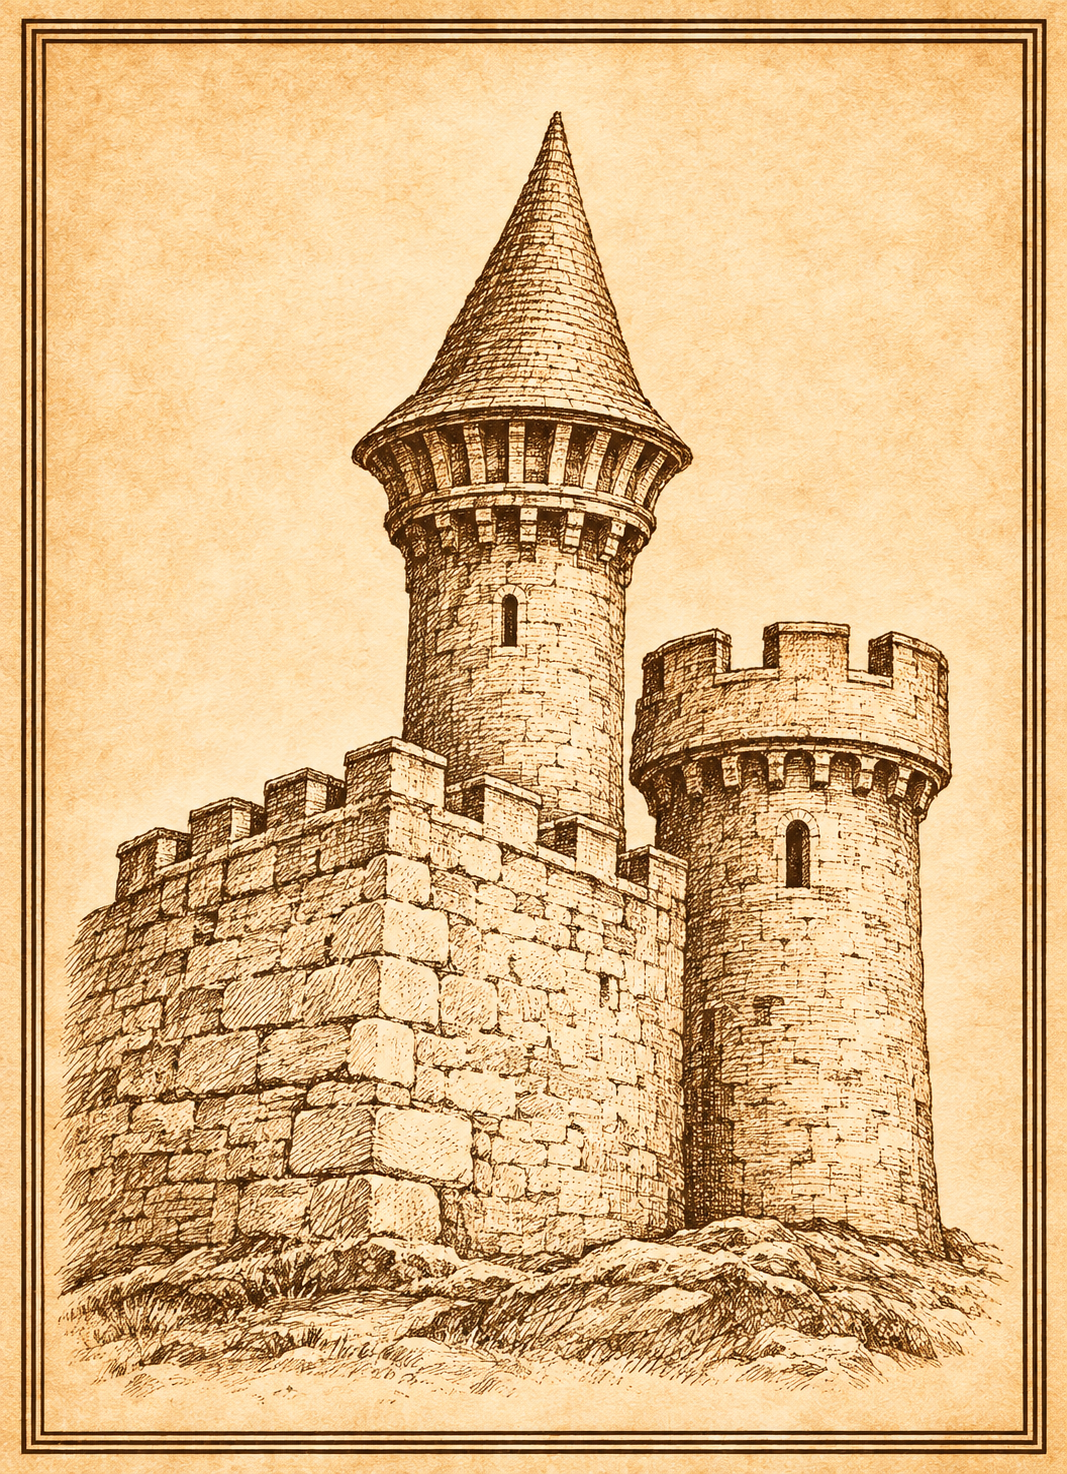
\includegraphics[width=0.34\textwidth]{imgs/005}
\end{center}

\clearpage

\begin{center}
    {\Large\itshape Alban pendant la guerre de Cent Ans}
\end{center}

\vspace{1.5em}

% Le bord gauche du scan est rogné : les débuts de plusieurs lignes
% ont été reconstitués lorsque le contexte et les fragments visibles le permettent.
\noindent Peu de renseignements nous sont parvenus sur la 1\textsuperscript{ère} partie du XIV\textsuperscript{ème} siècle. On note au passage qu'en 1342, un « Frédalen de Lumbenchir »\footnote{Aucune trace de cette personne n'est retrouvée dans les manuels classiques d'histoire. Est-ce une mauvaise transcription, ou bien un nom local que l'on ne trouve que dans les archives locales? Cela mérite d'être tiré au clair.} est seigneur d'Alban. Est-ce par ses soins qu'Alban s'organise en poste avancé en sentinelle de la région albigeoise ? La chose est possible. En fait, on n'a pas seulement à se défendre contre les Anglais mais aussi contre des bandes de maquisards multiples. Les comtes d'Armagnac, maîtres du Rouergue, les comtes de Foix qui sont en même temps vicomtes de Lautrec, les ducs de Berry et d'Anjou, qui sont gouverneurs du Languedoc, vident leurs querelles au détriment des populations. Les troupes de ces grands seigneurs féodaux sont, avec quelques militaires de métier, un ramassis de pillards et de brigands. Ces armées hétéroclites occupent les châteaux qui leur serviront de repaires. Ils pillent les campagnes, détroussant les uns, malmenant les autres. C'est alors que le rôle d'Alban comme sentinelle avancée et gardienne de la paix se manifeste. Il faut organiser la défense derrière les remparts, le cas échéant, traiter avec le chef ennemi, obtenir son éloignement, ne fût-il que momentané pour faire la moisson ou les vendanges.

\vspace{0.8em}

\noindent En 1360, les consuls d'Albi envoient un homme de confiance aux consuls de Trébas pour s'informer du passage des 500 hommes d'armes du Comte d'Armagnac.

\clearpage


\begin{center}
    {\Large\itshape Alban pendant la guerre de Cent Ans}
\end{center}

\vspace{1cm}

À quelque temps de là, Albi est informé que des bandes inconnues
occupent Villeneuve du Tarn. En mars 1361, les consuls d'Alban et
ceux de Villefranche avisent Albi à se tenir sur ses gardes.
Deux mois après, les consuls d'Albi envoient des émissaires
s'informer auprès des consuls d'Alban.

\medskip

En 1362, châteaux et bourgs des environs tombent entre les mains
de tous ces pillards. Massals, Miolles, Saint Jean de Janes,
Massuys, Curvalle, Trébas, Gaycre, Aygou, Padiès, Rosières,
Tanus\ldots

\medskip

En septembre 1368, Alban tombe aux mains des compagnies de
Provence, puis c'est le tour de Villefranche, et le 29 septembre
de cette même année, elles entrent dans les faubourgs d'Albi.

\medskip

Un observateur était envoyé, en juillet 1370, pour
« espiar »\footnote{Épier.} et s'informer sur les troupes qui venaient de
franchir le Tarn au bac de Trébas.

\medskip

Un an après, en 1371, au mois de mars, le trésorier du comte
d'Armagnac est à Alban. Un sergent nommé « Lyéric Davy »
envoyé par les consuls d'Albi était venu l'y rejoindre,
pour réclamer une paire de draps qui avaient été prêtés
et n'avaient pas été rendus.

\clearpage

% Page 030 — Alban pendant la guerre de Cent Ans
% Transcription fidèle de la page fournie.
% Les graphies et formulations du document ont été conservées.

\begin{center}
    {\Large\itshape Alban pendant la guerre de Cent Ans}
\end{center}

\vspace{1.5em}

\noindent
Comment le trésorier du comte d'Armagnac séjournant en ce mois de mars 1371 à Alban,
se tira-t-il de ces « vilains draps » ? L'envoyé des consuls d'Albi retourna-t-il
bredouille ? Peut être heureux de n'avoir pas été molesté par les soudards de ce
grand féodal ? On ne sait.

\medskip

\noindent
Ce qui est sûr, c'est que la guerre n'a apporté que des ruines. Alban s'est tiré
d'affaire sans, apparemment trop de mal. Mais en cet an 1371, la famine sévit et
bien des gens meurent de faim, et la guerre n'est pas finie. En 1380, les consuls
albanais écrivent à ceux d'Albi pour les renseigner sur des mouvements de troupes.
D'Alban, Bernat Domergue, en juin 1381, cours à Albi, on n'a plus le temps d'écrire.
Ça presse. Les Albigeois sont prévenue par notre concitoyen qu'un certain Bénézet,
Capitaine de routiers vient d'occuper Pousthomy, Montfranc, Trébas. En 1382, on
trouve ce brigand confortablement installé à Saint Jean de Janes. Il ne l'évacue
que contre rançon. Le château de Jaufin est pris et évacué en 1384 dans les mêmes
onéreuses conditions. Les dégâts sont tels dans la région d'Alban que sur
19 paroisses englobées dans l'archiprêtré de Nougaret (nous dirions doyenné
aujourd'hui), 7 paroisses sont exonérées d'impôts. Notre Dame d'Alban ne paie que
15 sols aux collecteurs pontificaux. Le Truel, Carménel, Ainestères, Saint Pierre
d'Alban, Massuyès, Ambialet, Villeneuve ne paient rien. C'est la dèche généralisée.

\clearpage

% Page 034 — Alban pendant la guerre de Cent Ans
% Transcription de la page fournie.
% La pagination de travail suit le classement retenu par l'auteur du projet.

\begin{center}
    {\Large\itshape Alban pendant la guerre de Cent Ans}
\end{center}

\vspace{1.5em}

\noindent
Après Paulin, c'est Curvalle qui, presque à la même date, va être victime à son tour
du brigandage. En effet, en mai 1384, un chef de bande nommé Espagnolet s'empare par
deux fois du château de Curvalle et met en coupe réglée le pays environnant. Les
méfaits sont si grands qu'il faut avoir recours aux forces royales pour se débarrasser
de cet encombrant personnage. En mai 1385, une armée royale commandée par le Seigneur
Gaucher de Passac arrive en Albigeois. Les Seigneurs du voisinage apportent leur
concours pour grossir la troupe. Celle-ci est approvisionnée par Albi. En juin 1385,
elle traverse Alban et va mettre le siège devant le château de Curvalle. Cela ne va
pas tout seul. Ce n'est qu'en octobre que la petite place forte est prise. Tous les
brigands qui s'y sont réfugiés sont pendus haut et court et séance tenante. Pendant
toutes les opérations du siège, les convois de vivres venant d'Albi ont passé par
Alban. On devine que tout ce va et vient n'a pas toujours été de tout repos pour nos
ancêtres Albanais. Le chroniqueur Froissart a raconté très pittoresquement les
péripéties de ce siège. (Les érudits y trouveront plaisir).

\medskip

\noindent
Cette fin de siècle n'est pas de tout repos. Albi s'inquiète et ses consuls viennent
se renseigner auprès de ceux d'Alban. Une fois de plus, des hommes d'armes ont occupé
Pousthomis. Une première démarche a eu lieu en avril 1387. En octobre de la même
année, deux consuls d'Albi arrivent chez nous pour obtenir des renseignements. La
guerre est à nos portes. Ces deux magistrats ont nom Gaudetru et Clergue. Ils vont
se rendre à cheval jusqu'à Nîmes pour y débattre des affaires de leur ville. Ils
sont de retour en nos murs douze jours après. En mai 1388, Clergue renouvelle sa
chevauchée et ne met que dix jours pour ce voyage éclair Albi-Nîmes-Albi.

\clearpage

% Page 32 du document source
% Transcription provisoire — à relire et corriger si nécessaire.

\begin{center}
    {\Large\itshape Alban pendant la guerre de Cent Ans}
\end{center}

\vspace{1.5em}

En septembre 1392, Alban reçoit Hélias de Vern, procureur du chapitre
Sainte Cécile d'Albi. Les consuls albigeois envoient deux sergents le
rejoindre. Ils sont porteurs d'un acte de procédure. Ces personnages ne
font que transiter par Alban. Ils se rendent dans le bas Languedoc. Et
ceci prouve l'importance de cette voie
de grand trafic à cette époque, de la route Aix -- Montauban sur laquelle
Alban se trouve comme un point d'étape apprécié.

\medskip

En cette fin de siècle, la famille des « Nougaret » semble prendre quelque
importance chez nous. Un Jacques de Nougaret est « viguier » (juge) à Albi
de 1396 à 1405.

\medskip

Au début du XV\textsuperscript{ème} siècle (Jeanne d'Arc naît en 1412),
une autre famille d'Alban, les De Moret, semble prendre de l'importance
dans notre coin. À cette date, en effet, Jehan de Moret prête serment pour
un fief noble qu'il détient dans la juridiction d'Alban. Et vingt ans
après en 1433, un Dominique de Moret nous est signalé comme marchand et
notable de notre cité. En 1450, nous apprenons qu'il fait commerce de fer
-- de ce fer qu'on extrait des « ferrières » de Paulin. Ce qu'on appelle
encore la Mouline (où résidait jadis ce brave Louis Fages) comportait en
fait deux moulins : l'un « drapier » parce qu'on y devait faire de la
toile ; c'était la « Mouline Bergan », et l'autre au-delà du ruisseau
« la Mouline Ferran », où se faisait le traitement des minerais de fer…
Aujourd'hui, il ne reste plus que le souvenir de ce temps passé, puisque
la « Mouline » n'a plus d'habitants.

\clearpage

% Page 33 du document source
% Transcription provisoire — à relire et corriger si nécessaire.

\begin{center}
    {\Large\itshape Alban au XV\textsuperscript{ème} siècle (suite)}
\end{center}

\vspace{1.5em}

Une autre notabilité, Paulin Limozin, achète à Armand de Rames,
commandeur des hospitaliers de Rayssac, des terres, des bois et des prés,
sis à Montredon, en 1447. Et c'est ainsi qu'un jour sera fondée sur ces
terres la chapellenie de Sainte Anne. Avec les revenus de la métairie de
Négremontet, entre le rec de l'Espazet et le chemin de la Tapie à Alban
jusqu'au rec de Fangouse et les prés de la Maye, devront être assurées à
perpétuité deux messes chaque semaine au bénéfice des donateurs. Trois
siècles après, les biens de la dite chapellenie seront cédés pour 1125
francs (de l'époque), le 17 février 1792 à Marcel Cros de Carménel qui les
avait lui-même achetés à Bonnet (de Carménel). Ce dernier les avait
acquis, lors de la vente des biens nationaux (biens confisqués par les
révolutionnaires) par les administrateurs au district d'Albi.

\medskip

Il se pourrait donc que les tènements plus ou moins en copropriété des
habitants de Carménel (en patois « patus ») soient peut-être, les biens
qui assuraient cette fondation de la chapellenie Sainte Anne. La Croix
qui a été dressée en ces parages, ces derniers temps, au sommet de la côte
de Fangouse et à la limite de terrains plus ou moins en friche, rappelle
ce passé. C'est la Croix de Sainte Anne, vocable que portait la susdite
chapellenie (chapellenie Sainte Anne). Si seulement, tous les ans, chaque
habitant de Carménel se donnait la peine d'y planter une sapinette, dans
vingt ans, il y aurait aux portes d'Alban un magnifique bois… à portée de
la main… et rentable.

\clearpage

% Page 34 du document source
% Transcription provisoire — à relire et corriger si nécessaire.

\begin{center}
    {\Large\itshape Alban au XV\textsuperscript{ème} siècle (suite)}
\end{center}

\vspace{1.5em}

En 1691, le curé de Notre Dame d'Alban, « Mestre » (Docteur en
théologie) Jean Alary, recteur, sentant sans doute sa fin prochaine,
céda le 13 mars 1691, les revenus de cette chapellenie dont il avait la
jouissance, à Pierre Amig, prêtre habitant Bazuéjouls (ou Bazuéjoulet ?)
à charge naturellement d'assurer deux messes par semaine.

\medskip

Le curé Jean Alary qui, en 1671 (il était arrivé en 1669), avait fait
graver, sans doute au-dessus de son presbytère, la devise : \textsc{A Dieu
seul}, avec un cœur servant de trait d'union à ces deux mots (\textit{Soli
Deo}), mourut effectivement quelque temps après avoir fait cette
donation. La pierre portant gravés son nom et sa devise a été conservée
et se trouve sous le banc de pierre, à droite, devant la façade de
l'église. On peut peut-être signaler que la présence d'un cœur dans la
devise s'expliquerait assez facilement, s'il y avait là un écho des
apparitions du Sacré Cœur à Sainte Marguerite Marie. Effectivement, les
révélations faites à la Sainte sont de ce temps-là.

\clearpage

% Page 35 du document source
% Transcription provisoire — à relire et corriger si nécessaire.

\begin{center}
    {\Large\itshape Alban au XV\textsuperscript{ème} siècle (suite)}
\end{center}

\vspace{1.5em}

En cette même année 1447, Bertrand Rauly d'Alban, fait hommage au comte
de Castres, pour un fief qu'il tient noblement dans le lieu d'Alban. Voilà
comment cette reconnaissance de possession s'accomplissait, si du moins
nous en croyons un hommage semblable rendu en 1443 à Philippe Jean de
Rabastens, seigneur de Paulin.

\medskip

Le requérant\footnote{L'emploi dans ce contexte mérite vérification.}, à genoux, tête découverte, sans ceinture à la taille,
mettait ses mains entre les mains de celui à qui il rendait hommage :
son suzerain. Le vassal, selon le texte latin, se tenait « genibus flexis,
sine capucis et zona, junctis manibus suis inter manus ipsius domini... ».

\medskip

Un événement plus important, du moins au point de vue ecclésiastique,
c'est regroupement de paroisses ordonné en ce début de siècle par
Monseigneur Robert Dauphin, évêque d'Albi. Négremont se voit dépossédé,
au bénéfice de Notre Dame d'Alban, de son titre d'Archiprêtré (nous
disons aujourd'hui « doyenné »). Le Pape Eugène IV, le 8 janvier 1438,
confirme la décision de l'évêque… Mais le dernier Archiprêtre de
Négremont recevra en compensation une rente viagère. (De nos jours, on
se contente généralement de coiffer le « démissionné » de quelque titre
plus ou moins honorifique… et encore… ne comportant pas de soulagement
en espèces sonnantes et trébuchantes… Autres temps… autres mœurs…).
Quant aux revenus de la paroisse de Négremont, alors 2000 livres, ils
devront assurer le traitement du successeur devenu simple « Vicaire
perpétuel », et payer en partie l'entretien des enfants de chœur de la
cathédrale Sainte Cécile d'Albi.

\clearpage

\begin{center}
    {\Large\itshape Alban au XV\textsuperscript{ème} siècle (suite)}
\end{center}

\bigskip

Ainsi, Saint Martin de Négremont finira par céder le pas à Notre Dame d'Alban qui devient successivement « chef lieu de Claverie » (une ferme porte encore sur la paroisse de Négremont ce nom de « La Claverie »), puis chef lieu de district et enfin de Doyenné.

On s'aperçoit que quelques siècles plus tard, les revenus de ce groupe de paroisses ne sont pas négligeables. En effet, le 13 juin 1721, Monseigneur de la Croix de Castries, évêque d'Albi, donne la jouissance des fruits décimaux de la claverie d'Alban -- et cela pour six ans -- à Maître Jean Dizarn, sieur de la Balme (habitant Coupiac) pour une redevance de 6000 livres : 920 en sont perçues à Saint Pierre d'Illergue, 1721 et 5 sols à Massals et Paulin, 854 à Massuèyes, 660 à Bonneval, 1450 à Teillet, 700 à Saint Jean du Salès. Quant aux « fruits décimaux » de Saint Jean de Janes, c'est le Grand Séminaire d'Albi qui en bénéficie.

À l'heure actuelle, le Doyenné Alban-Valence-Massals-Trébas-Teillet est beaucoup plus étendu géographiquement, mais ne comporte aucun revenu pour le titulaire (dommage !!!). Monsieur le Doyen de N.D. d'Alban.

\clearpage

\begin{center}
    {\Large\itshape Alban au XV\textsuperscript{ème} siècle (suite)}
\end{center}

\bigskip

En remontant dans le temps, nous aurions pu assister au mariage de noble Raymond de Peyrole d'Ambialet, avec Giscarde de la Roque, célébré le 30 janvier 1461 dans l'église du Travet (Bertrand de la Roque étant le seigneur de ce fief)... L'acte de mariage ne fut enregistré par le notaire de Valence, Maître Bénet que le 7 février 1475. Ce qui nous y intéresse, c'est qu'un albanais, Dominique de Moret, qui s'est enrichi dans le commerce du fer (rappelez-vous qu'il y a une mouline ferran), est témoin à la signature du contrat et que le notaire écrit à son sujet en latin D. de Moréto de Albanio (le mot est orthographié Alba NHO). Et ceci pourrait bien sembler un écho de l'accord passé deux siècles avant entre l'évêque d'Albi et le Père Abbé de Saint Benoît de Castres où il est effectivement question de Ecclesia Sanctae Marie de ALBANIO, et confirmerait d'une certaine façon l'hypothèse émise de l'appellation non pas de Notre Dame d'Alban mais de Notre Dame « des ALBANS » (les Albans étant une tribu gauloise qui aurait essaimé quelques siècles avant Jésus Christ et aurait fondé sur les rivages de l'Adriatique l'actuelle République d'Albanie). Ceci écrit pour le panache des actuels Albanais d'Alban. À cette date de 1475, les de Moret sont coseigneurs de Nougaret avec Bertrand de St Pol de Bonneval.

\clearpage

\begin{center}
    {\Large\itshape Alban en fin de siècle (XV\textsuperscript{ème})}
\end{center}

\bigskip

En cette fin de de XV\textsuperscript{ème} siècle, la paix semble donc bien assise. Aussi, en 1483 (nous sommes sous le règne de Charles VIII), Jean d'Armagnac, qui avait dû s'exiler tandis que son frère avait porté son cou sur le billot, veut réintégrer son évêché. Mais cette entrée dans la ville épiscopale de Castres est l'occasion de troubles. Partout, on se soulève contre celui qui a été imposé par le gouvernement royal comme gouverneur de Castres : Foffille de \footnote{nom illisible}. Et notre cité n'est pas la dernière à lever l'étendard de la révolte. La barre recommence. Ces « Albans » ont du sang de Vercingétorix dans les veines. César ne disait-il pas que si les Germains combattaient pour la rapine (ad praedam), les Gaulois, eux, c'était pour la liberté (pro libertate). Pauvres « Albans » de ce temps-là. L'affaire tourna mal pour eux. Bollille de Juge, après s'être emparé de Viane, prit d'assaut la petite place forte d'Alban. La cité rebelle fut pillée consciencieusement. Même son église ne fut pas épargnée. C'était en l'an 1484.

À part cet incident malheureux, il ne reste pas grand chose à glaner de notre histoire pour satisfaire notre curiosité. Citons cependant une délimitation entre les territoires de la paroisse N.D. d'Alban et ceux de St Michel de la Besse (actuellement la ferme St Michel, non loin du rocher de ce nom). Figurent dans l'acte passé devant Me Laurent, notaire : le représentant du chapitre de la cathédrale Sainte Cécile d'Albi à savoir le nouveau prieur de Négremont, pour le monastère St Benoît de Castres, son prieur, noble Raymond qu'accompagne Pierre ?alvan\footnote{Illisible} qui est de Castres. La limite fixée du côté du tènement appelé « lou Puech de la Bouyssière » (ne serait-ce pas ce qu'on appelle au roc des Anglais : la Puyssière ?...), confrontait vers le levant le château de Nougaret, situé au dessus du chemin d'Alban à Saint-André. Cette partie devait appartenir au prieur de Saint-Benoît, donc à l'abbaye, et la partie opposée située dans la juridiction d'Ambialet devait appartenir au chapitre cathédral de Ste Cécile d'Albi.

\clearpage

\bigskip

Ceci peut permettre de penser que le susdit château de Nougaret pouvait bien se situer sur ce petit plateau délimité par l'actuel chemin de Saint André et la route de Villeneuve non loin du « Castellus » dont le nom de « CASTELLAS » rappellerait précisément l'existence de cette demeure féodale aujourd'hui disparue.

Pour mémoire, auraient été à cette époque « coseigneurs » de la baronnie d'ALBAN, en même temps que les « de Moret », les « de Vernhette » qui figurent sous ce titre de coseigneurs d'Alban dans une étude généalogique aveyronnaise. Notre documentation actuelle ne permet ni d'infirmer, ni de confirmer cette assertion... Il est vrai, près de trois siècles après, ce qui est bien loin, on trouve comme vicaire (curé) à Saint Michel de Saint Léon (aujourd'hui appelé St Michel de Léon), un Jean Vernhet.

\clearpage

% Page 41 — Alban au temps de François 1er

\begin{center}
  {\Large\itshape Alban au temps de François 1\textsuperscript{er} (XVI\textsuperscript{ème} siècle)}
\end{center}

\vspace{1em}

\lettrine{U}{ne} période paisible : cette première moitié du XVI\textsuperscript{ème} siècle. Pour notre coin de montagne, les archives nous livrent le nom de quelques personnalités et font état d’une réorganisation tant au point de vue politique que religieux de ce terroir.

\medskip

Parmi les ecclésiastiques de cette époque, on trouve comme Prieur de N.D. d’Alban en 1505 un Raymond Guittard ; un peu plus tard, en 1508, c’est un Bertrand de Solages. (Les de Solages ont encore aujourd’hui dans leur famille plusieurs prêtres : Monseigneur Bruno de Solages, ancien recteur de l’Institut Catholique de Toulouse, François de Solages, curé de St Jean de Tartage à Gaillac, Hugues de Solages, curé de Cuq et de Serviès, etc…). Un ancien curé de Courris est signalé comme prieur de N.D. d’Alban en 1551 ; il s’agit de Jean de Moret. Ces de Moret illustrent particulièrement notre histoire locale. Raymond Gausseran est bien nommé en 1545 comme prêtre à N.D. d’Alban, mais en était-il curé ? On ne sait.

\medskip

\lettrine{O}{n} désigne communément comme fondateur de la « chapellenie de St Laurent » en 1516, un « Louis de Moret ». Il semble qu’à cela il y ait une petite difficulté, puisque déjà, le 14 juin 1457, on trouve un Jean Cathala au « Mas de la Cappélanyé » (actuellement la ferme de Capel-le-Bas, sous la nouvelle gendarmerie). On peut peut-être penser que Louis de Moret n’a fait qu’améliorer une fondation existante en la dotant de biens plus importants. A ce moment-là (en 1516), la chapellenie joint d’un immeuble dans Alban même et aux alentours du « mas » d’un pré dit « de la Cappélanyé ». Ce dernier confronte le hameau de la Drèch alors appelé « Calm », la route d’Alban à St Sernin et le rec (ruisseau) de la Cappélanyé. Les revenus de ces biens servaient à payer les honoraires des messes acquittées pour la famille des de Moret de Nougaret dont l’un d’eux était seigneur de la baronnie d’Alban.

\clearpage

% Page 42

\lettrine{U}{n} autre membre de cette famille, Jean de Moret, qui est bénéficier de Ste Cécile d'Albi (quelque chose comme chanoine titulaire), est bénéficiaire de la « Rectorie du Puy Saint Georges, près de Valdériès, et il l'arrente le 16 juin 1529 pour le compte de François de Lautrec pour la somme de 400 livres. On le trouve encore à Sainte Cécile en 1540. Un Jacques de Moret nous est signalé le 11 janvier 1567 dans un accord passé avec Antoine Laveygne. Pierre de Mammesse (orthographe incertaine) se reconnaît débiteur le 9 mai 1580 à l'égard de Pierre de Moret. Le débiteur est un notable puisque lieutenant principal dans le Castrais. La même année, un Antoine Caussé achète un cheval pour 55 écus et Louis de Moret, le soi-disant fondateur de la Chapellenie. Un autre de Moret, un peu plus tard en 1604 et le 3 juillet, se trouve être le prévôt de St Salvy d'Albi et il prétend devoir jouir d'une rente de 50 écus d'or à prendre sur les revenus du prieuré de Cambon et de Montels (son annexe) et il exhibe par devant notaire une lettre du Pape Clément VIII qui le fait bénéficier de cette rente....

\medskip

Quand, en 1945, fut révisé notre cadastre, on eut pour ce faire, des administrateurs ignorant notre patois languedocien. C'est un peu regrettable, car ne connaissant pas l'occitan, ils massacrèrent quelque peu les noms, les vocables et ils appelèrent le « rec de la Cappélanyé » « ruisseau de la Chapelaine ». Ceci sent le roman -- ce n'est pas très méchant et c'est bien savoureux, mais c'est : « Ruisseau de la CHAPELENIE ».

\clearpage

% Page 43 — Alban : XVIème siècle (début)

\begin{center}
  {\Large\itshape Alban : XVI\textsuperscript{ème} siècle (début)}
\end{center}

\vspace{1em}

\lettrine{S}{i} les « de Moret » font parler d'eux en ce début de XVI\textsuperscript{ème} siècle, par le rang social qu'ils occupent, ainsi Etienne de Moret en 1545 est lieutenant du roi pour la baronnie d'Alban, d'autres familles vont aussi prendre importance. Un acte du 12 octobre 1537 fait état de « noble François Caudière », fils d'Antoine, d'Alban, vendant à Bernard Olm habitant la Mouline Ferran, un vignoble qu'il a à Malagousse (dans les parages de l'actuel Parrot). Mais c'est surtout la famille des « de Passemar » qui va s'assurer la main-mise sur le pays. Le 3 juillet 1561, Guillaume de Passemar, marchand d'Alban, achète à M. de Candols toutes les rentes de la paroisse de Massals et celles des masages (hameaux) d'Oulas, des Escombrazes, de la Rode, de la Bartabié, de Pomardelle, de Tels, de la Fanguezié, de la borie des Coubès, de la Tapie, de Margou, de la Besse, de Tessonière, des Estrébols, de Bordes, de Cantarrane, du mas del Bosc, des Thérondeis, le tout pour 600 livres. Dans le cadastre de 1598, nous verrons ce « noble Guillaume de Passemar », seigneur de Cantelauze, venir en tête de liste après Notre Dame de Piétat (N.D. d'Alban sous le vocable de N.D. de Pitié) après les Hospitaliers (successeurs des Templiers) après la Chapellenie de St Laurent fondée par les de Moret, mais avant Jacques de Moret.

\medskip

\lettrine{A}{u} civil comme au religieux, une réforme administrative est en train de s'opérer au commencement de ce XVI\textsuperscript{ème} siècle. Le comté de Castres a été directement rattaché à la couronne de France après la mort de Boffille de Juge. On peut donc dire d'une certaine façon qu'à ce moment de l'histoire, le roi François 1\textsuperscript{er} est seigneur baron d'Alban. En même temps, notre cité a pris rang de « chef lieu de Claverie », nous disons aujourd'hui tête de doyenné. La ville d'Alban a ainsi remplacé l'ancien archiprêtré de Négremont, dont le dernier archiprêtre a été démissionné en 1438. Cette « Claverie », notez qu'une ferme porte encore ce nom, vestige du passé, comprend 13 chapellenies (nous disons aujourd'hui : « fondations pieuses ») dont celle de la Cappélanyé dite de St Laurent dont les de Moret

\clearpage

% Page 44 — suite de « Alban : XVIème siècle (début) »

seraient les fondateurs et celle de Sainte Anne fondée en 1477 par Paulin Limouzin (ou Limouzi) le 28 janvier de cette année-là. La susdite famille des Lemouzy est encore à Alban en 1598, l'un d'eux Meric Lemouzy possède une terre à La Bessière (là où sont actuellement les Bascoul) confrontant le chemin d'Alban à Réalmont et le chemin d'Alban à la Berrière aux terres de Jean Valette.

\medskip

\lettrine{À}{ la} même époque, disparaît l'abbaye Saint Benoît de Castres que remplace en 533 le chapitre cathédral de la même ville. Et c'est à ce même chapitre cathédral que sera rattachée, au moins juridiquement, la paroisse de Notre Dame d'Alban.

\medskip

\lettrine{D}{e}puis le dernier pillage de 1484 qui a suivi la rébellion des Albanais contre le délégué royal Boffille de Juge, jusqu'à 1562, c'est presque quatre vingt ans de paix dont jouira notre pays. Est-ce en ce temps-là qu'Alban a pu compter jusqu'à 400 feux (soit au bas mot 2000 habitants) ? Le cahier des doléances de 1789 y fera allusion. Mais nos délégués municipaux n'ont-ils pas gonflé un peu trop le chiffre, un peu à la manière des Maires d'aujourd'hui, afin d'obtenir des subventions désirables ? La chose n'est pas invraisemblable. D'autant que le registre cadastral de 1598 ne fera état que d'un chiffre inférieur à soixante feux (ou familles).

\clearpage

\begin{figure}[htbp]
    \centering
    
\includegraphics[width=0.38\textwidth]{imgs/006}
\end{figure}

\clearpage

%\input{pages/028-quatrième-de-couverture}
%\clearpage

\end{document}
